% Heatmap discussion section for Smash paper
% Include with: % Heatmap discussion section for Smash paper
% Include with: % Heatmap discussion section for Smash paper
% Include with: % Heatmap discussion section for Smash paper
% Include with: \input{heatmap_section}

\subsection{Sensitivity Analysis: Coldness vs.\ Compressibility}
\label{sec:heatmap}

To understand how Smash's effectiveness varies with workload characteristics, we conducted a controlled experiment measuring RSS reduction across the full range of two key parameters: \emph{hot data fraction} (the percentage of allocated data that is actively accessed) and \emph{data compressibility} (how well the data compresses).

\paragraph{Methodology.}
We allocate 2\,GB of data and vary two parameters independently:
\begin{itemize}
    \item \textbf{Hot data fraction} (0\%--100\%): The percentage of pages that are continuously accessed during the cooling and serving phases. Cold pages remain untouched after initial allocation.
    \item \textbf{Data compressibility} (0\%--100\%): The fraction of each page filled with zeros (highly compressible) versus random bytes (incompressible). At 100\% compressibility, pages contain only zeros; at 0\%, pages contain random data.
\end{itemize}
We measure steady-state RSS after a 30-second cooling period and compare against a baseline using the system allocator.

\paragraph{Results.}
Figure~\ref{fig:heatmap} shows the RSS reduction achieved by Smash across all combinations of these parameters. The results reveal several important characteristics:

\begin{figure}[t]
    \centering
    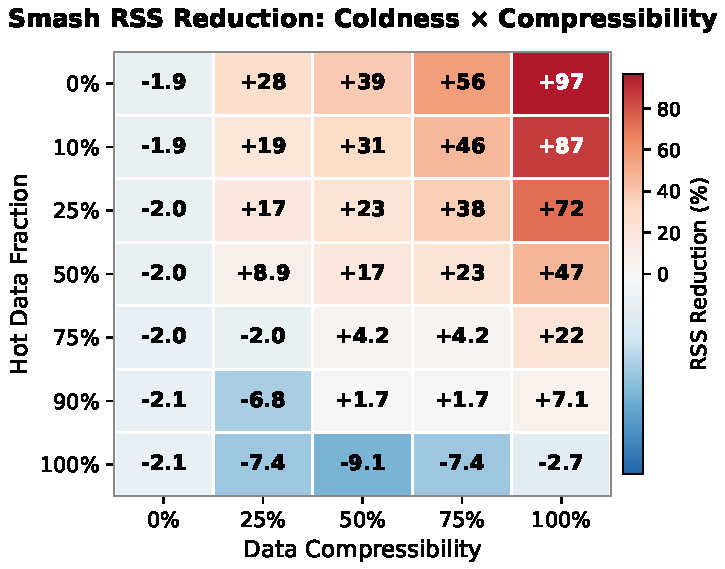
\includegraphics[width=\columnwidth]{figures/heatmap_2gb.pdf}
    \caption{Smash RSS reduction (\%) as a function of hot data fraction (rows) and data compressibility (columns). Positive values (warm colors) indicate RSS savings; negative values (cool colors) indicate overhead. With fully compressible cold data (top-right), Smash achieves up to 97\% RSS reduction. Incompressible data (left column) shows small overhead ($\sim$2\%) from Smash's metadata.}
    \label{fig:heatmap}
\end{figure}

\begin{enumerate}
    \item \textbf{Compressibility is the dominant factor.} Moving from left to right (increasing compressibility), RSS reduction increases dramatically regardless of the hot fraction. At 100\% compressibility with 0\% hot data, Smash achieves 97\% RSS reduction---compressing 2\,GB down to $\sim$69\,MB.

    \item \textbf{Cold data amplifies benefits.} For any given compressibility level, having more cold data (lower hot fraction) improves RSS reduction. At 75\% compressibility, RSS reduction ranges from 57\% (0\% hot) to 7\% (100\% hot).

    \item \textbf{Overhead is bounded.} With incompressible data (0\% compressibility), Smash incurs only $\sim$2\% overhead from its metadata structures, regardless of the hot fraction. This confirms that Smash's ROI model correctly avoids compressing pages that would not benefit.

    \item \textbf{The sweet spot is common.} Most real-world applications have significant amounts of both cold data and compressible data (strings, sparse structures, zero-initialized buffers). The center and upper-right regions of the heatmap---showing 20--90\% reduction---represent typical application behavior.
\end{enumerate}

\paragraph{Implications.}
This analysis explains why Smash achieves substantial RSS reductions on real applications like SQLite (44\% reduction), RocksDB (73\% reduction during cooling), and Redis (47\% reduction): these applications naturally exhibit both temporal locality (hot/cold separation) and data compressibility. Applications with purely random, always-hot data would see minimal benefit, but such workloads are rare in practice.


\subsection{Sensitivity Analysis: Coldness vs.\ Compressibility}
\label{sec:heatmap}

To understand how Smash's effectiveness varies with workload characteristics, we conducted a controlled experiment measuring RSS reduction across the full range of two key parameters: \emph{hot data fraction} (the percentage of allocated data that is actively accessed) and \emph{data compressibility} (how well the data compresses).

\paragraph{Methodology.}
We allocate 2\,GB of data and vary two parameters independently:
\begin{itemize}
    \item \textbf{Hot data fraction} (0\%--100\%): The percentage of pages that are continuously accessed during the cooling and serving phases. Cold pages remain untouched after initial allocation.
    \item \textbf{Data compressibility} (0\%--100\%): The fraction of each page filled with zeros (highly compressible) versus random bytes (incompressible). At 100\% compressibility, pages contain only zeros; at 0\%, pages contain random data.
\end{itemize}
We measure steady-state RSS after a 30-second cooling period and compare against a baseline using the system allocator.

\paragraph{Results.}
Figure~\ref{fig:heatmap} shows the RSS reduction achieved by Smash across all combinations of these parameters. The results reveal several important characteristics:

\begin{figure}[t]
    \centering
    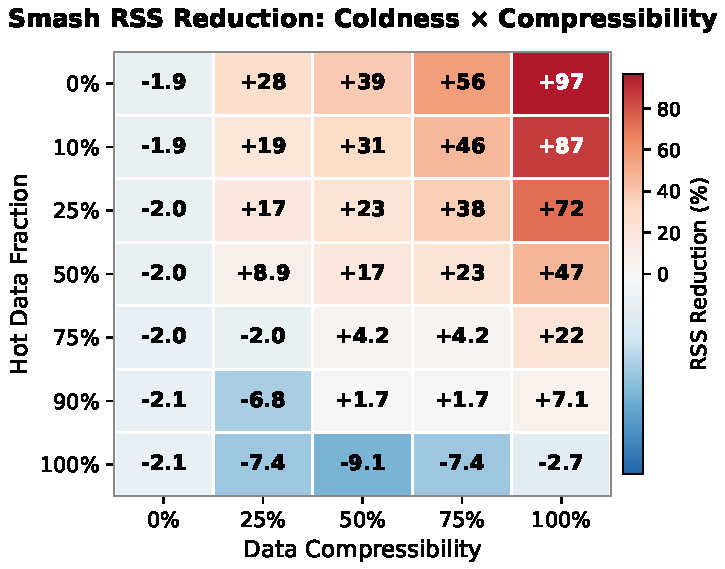
\includegraphics[width=\columnwidth]{figures/heatmap_2gb.pdf}
    \caption{Smash RSS reduction (\%) as a function of hot data fraction (rows) and data compressibility (columns). Positive values (warm colors) indicate RSS savings; negative values (cool colors) indicate overhead. With fully compressible cold data (top-right), Smash achieves up to 97\% RSS reduction. Incompressible data (left column) shows small overhead ($\sim$2\%) from Smash's metadata.}
    \label{fig:heatmap}
\end{figure}

\begin{enumerate}
    \item \textbf{Compressibility is the dominant factor.} Moving from left to right (increasing compressibility), RSS reduction increases dramatically regardless of the hot fraction. At 100\% compressibility with 0\% hot data, Smash achieves 97\% RSS reduction---compressing 2\,GB down to $\sim$69\,MB.

    \item \textbf{Cold data amplifies benefits.} For any given compressibility level, having more cold data (lower hot fraction) improves RSS reduction. At 75\% compressibility, RSS reduction ranges from 57\% (0\% hot) to 7\% (100\% hot).

    \item \textbf{Overhead is bounded.} With incompressible data (0\% compressibility), Smash incurs only $\sim$2\% overhead from its metadata structures, regardless of the hot fraction. This confirms that Smash's ROI model correctly avoids compressing pages that would not benefit.

    \item \textbf{The sweet spot is common.} Most real-world applications have significant amounts of both cold data and compressible data (strings, sparse structures, zero-initialized buffers). The center and upper-right regions of the heatmap---showing 20--90\% reduction---represent typical application behavior.
\end{enumerate}

\paragraph{Implications.}
This analysis explains why Smash achieves substantial RSS reductions on real applications like SQLite (44\% reduction), RocksDB (73\% reduction during cooling), and Redis (47\% reduction): these applications naturally exhibit both temporal locality (hot/cold separation) and data compressibility. Applications with purely random, always-hot data would see minimal benefit, but such workloads are rare in practice.


\subsection{Sensitivity Analysis: Coldness vs.\ Compressibility}
\label{sec:heatmap}

To understand how Smash's effectiveness varies with workload characteristics, we conducted a controlled experiment measuring RSS reduction across the full range of two key parameters: \emph{hot data fraction} (the percentage of allocated data that is actively accessed) and \emph{data compressibility} (how well the data compresses).

\paragraph{Methodology.}
We allocate 2\,GB of data and vary two parameters independently:
\begin{itemize}
    \item \textbf{Hot data fraction} (0\%--100\%): The percentage of pages that are continuously accessed during the cooling and serving phases. Cold pages remain untouched after initial allocation.
    \item \textbf{Data compressibility} (0\%--100\%): The fraction of each page filled with zeros (highly compressible) versus random bytes (incompressible). At 100\% compressibility, pages contain only zeros; at 0\%, pages contain random data.
\end{itemize}
We measure steady-state RSS after a 30-second cooling period and compare against a baseline using the system allocator.

\paragraph{Results.}
Figure~\ref{fig:heatmap} shows the RSS reduction achieved by Smash across all combinations of these parameters. The results reveal several important characteristics:

\begin{figure}[t]
    \centering
    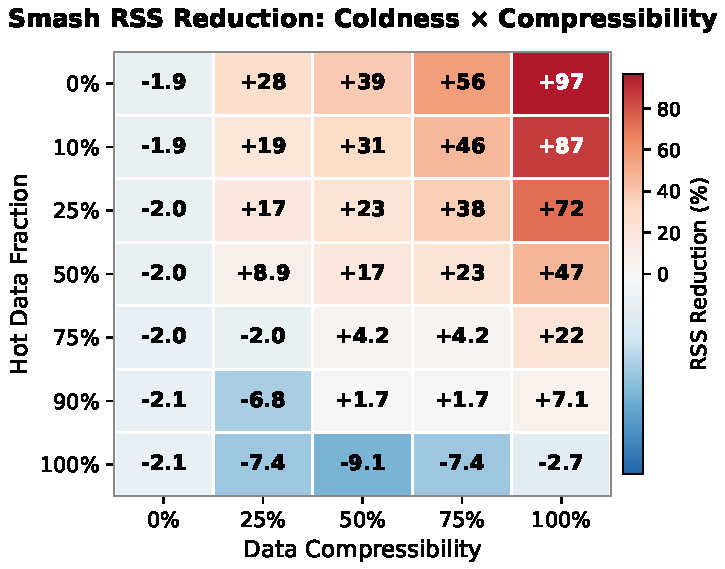
\includegraphics[width=\columnwidth]{figures/heatmap_2gb.pdf}
    \caption{Smash RSS reduction (\%) as a function of hot data fraction (rows) and data compressibility (columns). Positive values (warm colors) indicate RSS savings; negative values (cool colors) indicate overhead. With fully compressible cold data (top-right), Smash achieves up to 97\% RSS reduction. Incompressible data (left column) shows small overhead ($\sim$2\%) from Smash's metadata.}
    \label{fig:heatmap}
\end{figure}

\begin{enumerate}
    \item \textbf{Compressibility is the dominant factor.} Moving from left to right (increasing compressibility), RSS reduction increases dramatically regardless of the hot fraction. At 100\% compressibility with 0\% hot data, Smash achieves 97\% RSS reduction---compressing 2\,GB down to $\sim$69\,MB.

    \item \textbf{Cold data amplifies benefits.} For any given compressibility level, having more cold data (lower hot fraction) improves RSS reduction. At 75\% compressibility, RSS reduction ranges from 57\% (0\% hot) to 7\% (100\% hot).

    \item \textbf{Overhead is bounded.} With incompressible data (0\% compressibility), Smash incurs only $\sim$2\% overhead from its metadata structures, regardless of the hot fraction. This confirms that Smash's ROI model correctly avoids compressing pages that would not benefit.

    \item \textbf{The sweet spot is common.} Most real-world applications have significant amounts of both cold data and compressible data (strings, sparse structures, zero-initialized buffers). The center and upper-right regions of the heatmap---showing 20--90\% reduction---represent typical application behavior.
\end{enumerate}

\paragraph{Implications.}
This analysis explains why Smash achieves substantial RSS reductions on real applications like SQLite (44\% reduction), RocksDB (73\% reduction during cooling), and Redis (47\% reduction): these applications naturally exhibit both temporal locality (hot/cold separation) and data compressibility. Applications with purely random, always-hot data would see minimal benefit, but such workloads are rare in practice.


\subsection{Sensitivity Analysis: Coldness vs.\ Compressibility}
\label{sec:heatmap}

To understand how Smash's effectiveness varies with workload characteristics, we conducted a controlled experiment measuring RSS reduction across the full range of two key parameters: \emph{hot data fraction} (the percentage of allocated data that is actively accessed) and \emph{data compressibility} (how well the data compresses).

\paragraph{Methodology.}
We allocate 2\,GB of data and vary two parameters independently:
\begin{itemize}
    \item \textbf{Hot data fraction} (0\%--100\%): The percentage of pages that are continuously accessed during the cooling and serving phases. Cold pages remain untouched after initial allocation.
    \item \textbf{Data compressibility} (0\%--100\%): The fraction of each page filled with zeros (highly compressible) versus random bytes (incompressible). At 100\% compressibility, pages contain only zeros; at 0\%, pages contain random data.
\end{itemize}
We measure steady-state RSS after a 30-second cooling period and compare against a baseline using the system allocator.

\paragraph{Results.}
Figure~\ref{fig:heatmap} shows the RSS reduction achieved by Smash across all combinations of these parameters. The results reveal several important characteristics:

\begin{figure}[t]
    \centering
    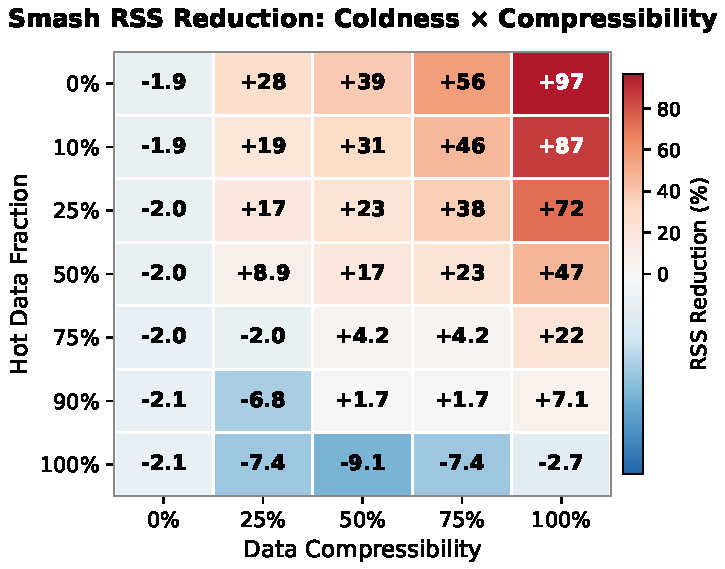
\includegraphics[width=\columnwidth]{figures/heatmap_2gb.pdf}
    \caption{Smash RSS reduction (\%) as a function of hot data fraction (rows) and data compressibility (columns). Positive values (warm colors) indicate RSS savings; negative values (cool colors) indicate overhead. With fully compressible cold data (top-right), Smash achieves up to 97\% RSS reduction. Incompressible data (left column) shows small overhead ($\sim$2\%) from Smash's metadata.}
    \label{fig:heatmap}
\end{figure}

\begin{enumerate}
    \item \textbf{Compressibility is the dominant factor.} Moving from left to right (increasing compressibility), RSS reduction increases dramatically regardless of the hot fraction. At 100\% compressibility with 0\% hot data, Smash achieves 97\% RSS reduction---compressing 2\,GB down to $\sim$69\,MB.

    \item \textbf{Cold data amplifies benefits.} For any given compressibility level, having more cold data (lower hot fraction) improves RSS reduction. At 75\% compressibility, RSS reduction ranges from 57\% (0\% hot) to 7\% (100\% hot).

    \item \textbf{Overhead is bounded.} With incompressible data (0\% compressibility), Smash incurs only $\sim$2\% overhead from its metadata structures, regardless of the hot fraction. This confirms that Smash's ROI model correctly avoids compressing pages that would not benefit.

    \item \textbf{The sweet spot is common.} Most real-world applications have significant amounts of both cold data and compressible data (strings, sparse structures, zero-initialized buffers). The center and upper-right regions of the heatmap---showing 20--90\% reduction---represent typical application behavior.
\end{enumerate}

\paragraph{Implications.}
This analysis explains why Smash achieves substantial RSS reductions on real applications like SQLite (44\% reduction), RocksDB (73\% reduction during cooling), and Redis (47\% reduction): these applications naturally exhibit both temporal locality (hot/cold separation) and data compressibility. Applications with purely random, always-hot data would see minimal benefit, but such workloads are rare in practice.
